%%%%%%%%%%%%%%%%%%%%%%%%%%%%%%%%%%%%%%%%%
%%% WP01
%%%%%%%%%%%%%%%%%%%%%%%%%%%%%%%%%%%%%%%%%

\tsubsubsection{WP05 - Open Diverse and Inclusive Science}

%%%%%%%%%%%%%%%%%%%%%%%%%%%%%%%%%%%%%%%%%
%%% Section content, please change!
%%%%%%%%%%%%%%%%%%%%%%%%%%%%%%%%%%%%%%%%%

\subsubsection*{Overview and Goals}

\begin{table}[H]
    \renewcommand{\arraystretch}{1.50}		
    \footnotesize   
    \begin{tabular}{*{3}{|p{0.10\textwidth}}|l|}
        \hline
        \rowcolor{mygray} \multicolumn{4}{|c|}{\textit{\color{white}Work Package Summary}} \\
        \hline
        \rowcolor{mylightergray} \textit{WP 5} & \cellcolor{white} 01 & \textit{Title of WP} & \cellcolor{white} Open Diverse and Inclusive Science \\
        \hline
        \rowcolor{mylightergray} \textit{Start} & \cellcolor{white} Mxx & \textit{End} & \cellcolor{white} Myy \\
        \hline
        \rowcolor{mylightergray} \multicolumn{4}{|p{0.978\textwidth}|}{\textit{Participating Organisations}} \\
        \hline
        \multicolumn{4}{|p{0.978\textwidth}|}{
            \hspace*{-0.75cm} 
            \begin{minipage}[t]{\textwidth}
    			\begin{itemize}
    			    \item WP Leader: Partner 1
    				\item Participants: Partner 2, Partner 3, Partner 4, Partner 5, Partner 6, Partner 7
    			\end{itemize} 
    			\vspace*{0.10em}
			\end{minipage}
        } \\
        \hline
    \end{tabular}
    \vspace{0.5em}\vfill
    \begin{tabular}{|p{0.978\textwidth}|}
        \hline
        \rowcolor{mylightergray} \textit{Goals} \\
        \hline
        \rowcolor{white} 
        \hspace*{-0.75cm} 
        \begin{minipage}[t]{\textwidth}
    		\begin{itemize}
    		    \item Goal 1
    			\item Goal 2
			    \item Goal 3
    		\end{itemize} 
    		\vspace*{0.10em}
		\end{minipage}        
        \\
        \hline
    \end{tabular}
    \vspace{0.5em}\vfill
    \begin{tabular}{|l|*{7}{>{\centering\arraybackslash}p{0.084\textwidth}|}}
        \hline    
        \rowcolor{mylightergray} \textit{Participant number} & \textit{1} & \textit{2} & \textit{3} & \textit{4} & \textit{5} & \textit{6} & \textit{7} \\
        \hline
        \rowcolor{white} \cellcolor{mylightergray}\textit{Participant short name} & Partner 1 & Partner 2 & Partner 3 & Partner 4 & Partner 5 & Partner 6 & Partner 7 \\
        \hline
        \rowcolor{white} \cellcolor{mylightergray}\textit{PM per participant} & xx & xx & xx & xx & xx & xx & xx \\
        \hline        
    \end{tabular}    
\end{table}

\subsubsection*{Status}

\todo{Briefly explain the status of the WP.}

\subsubsection*{Progress per Task}

\subparagraph{Task 5.2: Open Science } \mbox{}
\todo{Work In Progress}

Within WP5, the goal of the Task 5.2 is to provide new services to the users in order to achieve an improved and facilitated access to experimental dataset produced in Research Infrastructures. The services aims at improved FAIR data practices. This includes (1) a new data catalog (openNP), (2) an authentification and authorization (AAI) service and (3) a prototype of plateform for data access.

During the reporting period for the sub tasks, the main results are :
\begin{itemize}
    \item  release of the specification document of the openNP catalog under MS35.
    \item the AAI service based on INDIGO-IAM was published online (https://iam-eurolabs.ijclab.in2p3.fr/) and is now being used by the Virtual Access platform Theo4Exp of the EURO-LABS Project (Task 2.4) to authentify their users. To date, more than 250 users are registered and the services is used for the authentication various services (Theo4NP (Task of EURO-LABS), grafana monoriting services at GSI and GANIL) Promotion of the service to future user was achieved.
    \item Different data lake prototypes are being developed/tested based also in coordination with the ESCAPE Project and the PUNCH4NFDI project. The results from these prototypes combined with the other related activities like AAI, will lead to a federated infrastructure concept that will be implemented in FAIR and other infrastructures.
    \item An advanced training school on data management was organized under EURO-LABS WP5.4 and the HGS-HIRe doctoral school in Nov 2024. Lectures and Hands on material can be found in  : \url{https://indico.gsi.de/event/19808/}. The material produced by the school attendees was also published on the zenodo repository of the project. 
\end{itemize}

In addition, under Task 5.2, the Data Management Plan of the EURO-LABS project was reviewed and updated (D5.8).

Digital objects (reports, deliverables, communications, ...) produced by the project can be found on the zenodo repository of the project (\url{https://zenodo.org/communities/euro-labs}). 

\subparagraph{Task 5.3: Machine Learning (Month xx-yy)} \mbox{}


\todo{Work in Progress}

Within WP5, the Task 5.3 aims to use Machine Learning (ML) methods to improve beam characteristics, transport efficiency, and reproducibility of accelerator tuning, which will reduce the beam preparation time and thus the available time for the experiments. Accelerator laboratories worldwide are exploring a large variety of techniques to achieve this aim, from classical optimization and Bayesian optimization (BO) to reinforcement learning. One part of this automation effort is to provide a framework that allows machine experts, operators, and users to solve certain, focused optimization problems and to make these solutions reusable in an operational context. We call this project the “Generic Optimization Framework and Frontend”, or Geoff for short.  EURO-LABS finances one scientific staff
member at GSI for three years for deployment and implication of Geoff for improved beam delivery at EURO-LABS facilities.

The main result of Task 5.3 is the regular use of Geoff at two facilities, CERN (Switzerland) and GSI (Germany). Its successful application to improve accelerator tuning at GSI has been demonstrated in several dedicated beam experiments. The beam loss of the injection into the SIS18 synchrotron has been reduced from 40$\%$ to 15$\%$ in about 15 minutes, where manual tuning can take up to 2 hours. Geoff has also been successfully applied to the GSI Fragment Separator (FRS) for beam steering and focusing, see Figure~\ref{fig:wp5_frs}. In particular, the great flexibility of Geoff, allowing the integration of new and legacy control systems, has significantly facilitated and accelerated the application of ML methods at GSI. 

\begin{figure}
    \centering
        \begin{tikzpicture}
        \node[above] (vis) at (0.0, 0.0) {%
            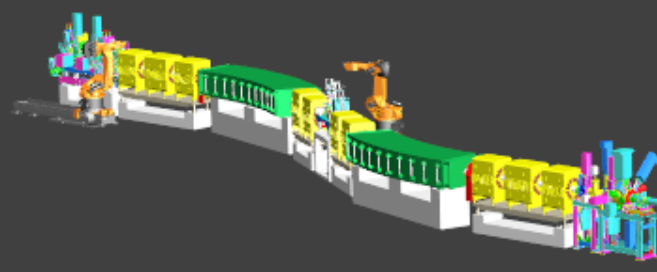
\includegraphics[width=0.45\textwidth]{graphics/wp5_gsi_frs_vis-3d.png}%
        };
        \node[below right] (obs) at (1.0, -1.0) {%
            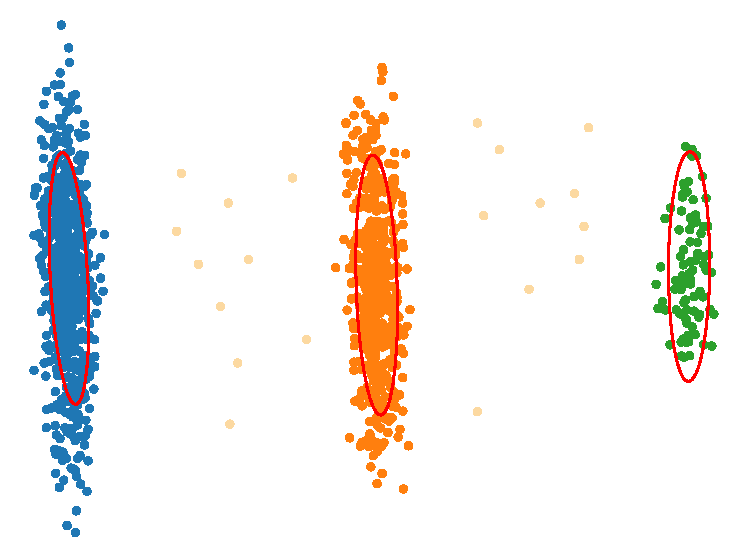
\includegraphics[width=0.20\textwidth]{graphics/wp5_gsi_clusters-speckled.pdf}%
        };
        \node[below left] (res) at (0.0, -0.7) {%
            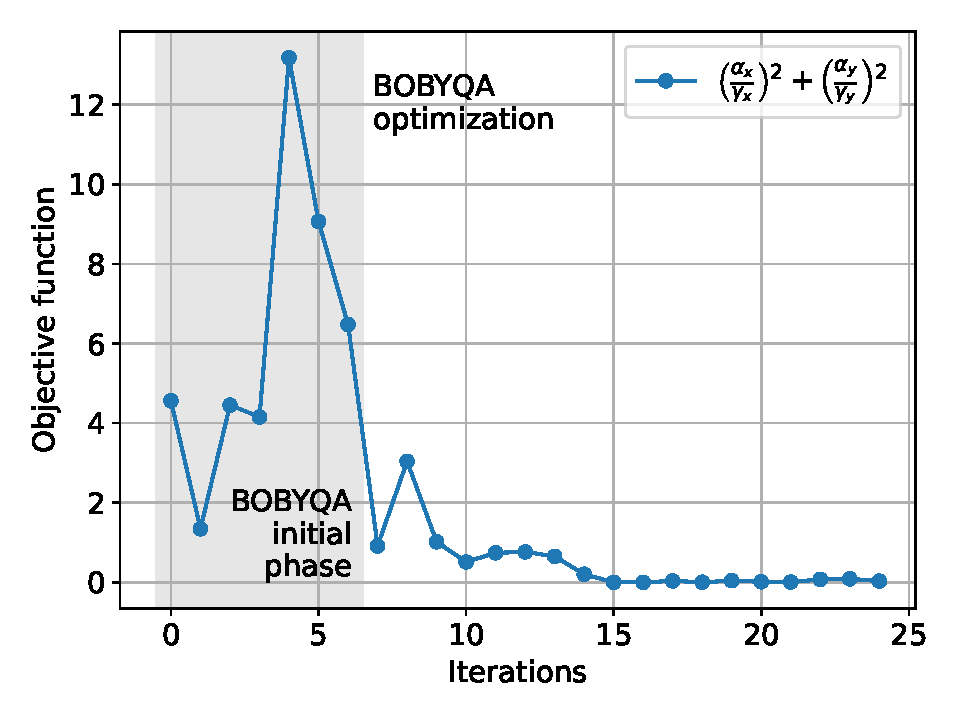
\includegraphics[width=0.31\textwidth]{graphics/wp5_gsi_bobyqa.pdf}%
        };
        \path[use as bounding box] (res.south west) (vis.north) (obs.south east);
        \begin{scope}[node font=\scriptsize\bfseries, above, inner sep=0]
            \node (vis title) at (vis.north) {Illustration of FRS Dispersive Area};
            \node (obs title) at (obs.north) {TPC Data Dnalysis};
        \end{scope}
        \node[
        draw=orange,
        ultra thick,
        circle,
        minimum width=1.2cm,
        minimum height=1.4cm,
        ] (quads) at (1.9, 0.9) {};
        \begin{scope}[->, >=Triangle, draw=blue, ultra thick, node font=\tiny]
            \draw (obs) -- (obs -| res.east)
            node[midway, above, align=center, text width=1.5cm, outer sep=3pt] {%
                evaluation of beam spot slope%
            };
            \draw (res.60) -- (quads)
            node[pos=0.6, text=white, above left, align=center, outer sep=auto] {%
                change\\quadrupole\\strengths%
            };
            \draw (quads) -- (obs title);
        \end{scope}
    \end{tikzpicture}
    \caption{Automatic online focusing for the GSI Fragment Separator (FRS) that uses the BOBYQA algorithm. The gray area in the left figure marks the initialization phase of the algorithm. Convergences has been reached after about 15 iterations. The objective function (left figure, legend) is a scalar measure of how vertical the U91+ beam spot is oriented (right figure). The BOBYQA algorithm optimizes the strength of the quadrupole magnets (top figure).}
    \label{fig:wp5_frs}
\end{figure}

The adaptation of Geoff to a laser-driven particle accelerator
at CEA (France) has started in  November 2024. A majority of the work will be carried out by the post-doctoral researcher financed by Euro-Labs in collaboration with GSI and CERN. The firts tests on the LPA-UHI100 facility ( part of the facilities offering beamtime through WP3) will start as soon as the final authorization to shoot full energy on target will be given by ASN (Nuclear Safety Authority)/CEA. 

\subparagraph{Task 5.4: Training (Month xx-yy)} \mbox{}

\todo{Briefly explain the progress of the task in context to the DoA.}
Within WP5, Task 5.4 aims to assure and improve the participation of new generations of scientists by the yearly organization of basic and advanced training schools, hosted by different beneficiary institutions of EURO-LABS, as well as the identification and partial support of other training events that are organized in Europe in order not to duplicate efforts. We have proposed to have four Basic Training School (BTS) and four Advanced Training School (ATS), and in addition to support events organized by Beneficiaries of EURO-LABS that fit the scope of our training Task 5.4.
So far we have organised two basic schools: BTS23 in September 13$^{th}$–23$^{rd}$, 2023, at IFIN-HH, Bucharest-Magurele, Romania ((https://indico.nipne.ro/event/246/) and BTS24 in June 18$^{th}$-27$^{th}$ 2024, in Warsaw, Poland(https://www.slcj.uw.edu.pl/en/bts24/), hosted by HIL and ICST, Warsaw and two advanced schools: ATSOA (Advanced training School on Operation of Accelerators in June 3$^{rd}$ -7$^{th}$, 2024, at CERN (https://indico.cern.ch/event/1357293/) and Advanced School on Open Science and Data Management in Nov. 24$^{th}$-27$^{th}$, at GSI/FAIR, Darmstadt, Germany (https://indico.gsi.de/event/19808/). All information about the school can be reached from the EURO-LABS web site. The details are also included in the deliverable D5.5 "Report on activities after 2 years, including follow-up from participants" (August 31, 2024). All of these schools were well attended by students and young researchers from Europe and other continents and were very much appreciated. The hosts asked the participants to answer questions that were later used to better organize the next events. 

Additionally, EURO-LABS has supported (co-sponsored) the “R-matrix school” in Edinburgh and the Nuclear Physics for Astrophysics NPA XI school in Dresden, Sep. 9-15, 2024. In its latest meeting TSB has approved tho organization of the remainder two BTS schools at CNA Seville in June 2025 and IFIN-HH in May 2026. TSB reviewed further requests for support (co-sponsorship) from The NIC XVIII school, Barcelona, June 2025, and the Carpathian Summer School of Physics, Sinaia, June 2025. Both requests were accepted and the events are being organized right now.


Currently we are working on the new edition of the advance school in accelerators, ATSOA25 that will take place in May 12$^{th}$-16$^{th}$ at CERN. We had 32 application and 20 trainees were selected. The basic School on Accelerator Applications, BTS25, will take place in Seville from 3rd to 9th of June[https://indico.cern.ch/event/1482911/]. The period for application close March 3rd.

All events organized or supported so far were very successful, based on the number of participants, and their positive feedback. The organizers and trainers, have seen how such events can be even better organized and planned to further increase the impact for the youngsters.
Below are some of the major feedback that was received:
- Hands-on events are most appreciated by trainees
- Diversity of equipment and installations used was well appreciated by those who are at the point     of choosing a career path for their upcoming careers.
- Basic Schools of 10-12 days long allow the trainees to work directly and to know each-other, 
We noticed that Younger scientists are the most appreciated trainers

\subsubsection*{Main Results and Achievements}

\todo{Briefly summarise the main results and achievements of the WP in context of the DoA.}
Activities under Task 5.4 started with the selection of a Training Scientific Board (TSB), completed by Feb. 2023. The activities that followed were in agreement with the initial proposal and overseen by TSB. Basic Training Schools (BTS) and Advanced Training Schools on Operation of Accelerators (ATSOA) were organized:

BTS23 at IFIN-HH, Bucharest-Magurele, Romania

BTS24, at HIL and INC, Warsaw, Poland

ATSOA24 at CERN, Geneve, Switzerland / France

ATSOSDM24 by GSI/FAIR, Darmstadt, Germany

ATSOA25, at CERN - organization in progress

BTS25 in Seville, Spain - organization in progress.

Two schools were co-sponsored in 2024 and two more were approved for sponsorship in 2025.
\subsubsection*{Deviations and Corrective Actions}

\todo{Briefly summarize any deviations and performed corrective actions of the WP in context of the DoA.}
Organizers asked the young participants to judge the events and activities they attended. They appreciated most the hands-on activities and that was strengthened. When confronted with applications from students from other continents (America, Africa) for which we feared we will not have sufficient funds, we have learned that the applicants could come with travel support from their home institutions. That enlarged the reach of the events and of EURO-LABS to the international communities. We have also learned that common extra-curricula activities bind very much the young participants and their hosts.
\subsubsection*{Milestones and Deliverables}

{\fontsize{9}{11}\selectfont
\begin{center}
  \begin{tabular}[t]{!{\color{mygray}\vrule}p{0.10\linewidth}!
  {\color{mygray}\vrule}p{0.60\linewidth}!
  {\color{mygray}\vrule}p{0.20\linewidth}!{\color{mygray}\vrule} } \hline
    \rowcolor{mycyan} & {\bf Title} & {\bf Status} \\ 

    \hline
    \cellcolor{mycyan}{\bf D5.1}: & All research  infrastructures videos completed & Achieved \\
    \hline
    \cellcolor{mycyan}{\bf D5.4}: & The new toolkit deployed at least two facilities and been used optimization  & Achieved \\
    \hline
    \cellcolor{mycyan}{\bf D5.5}: & Report on Training Activities after 2 years including followup from participants & Achieved \\ 
    \hline
    \cellcolor{mycyan}{\bf D5.8}: & Data Management Plan – Interim release  & Achieved \\ 
    \hline
  \end{tabular}
\end{center}
}

\subsubsection*{Project Meetings}

%  {\color{mygray}\vrule}p{0.40\linewidth}!

%%%%%%%%%%%%%%%%%%%%%%%%%%%%%%%%%%%%%%%%%